\subsection{OTFS-IM Design Objectives and Architecture}

This section introduces the role of OTFS-IM in the proposed system design. It clarifies why index modulation is applied in the delay-Doppler domain and how the resulting architecture extends the baseline OTFS model.

\subsubsection{Motivation and Design Objectives}

The baseline OTFS system developed in Chapter 3 places QAM symbols on all available delay-Doppler resource elements. This structure is suitable for time-varying multipath channels because the information symbols are represented in a domain where delay and Doppler effects can be described more naturally. However, the baseline OTFS transmitter uses only the symbol values themselves to convey information. The positions of the delay-Doppler resource elements are fixed and do not carry additional bits.

Index Modulation introduces a different way of using the same resource grid. Instead of activating every resource element, only a selected subset of positions is activated inside each transmission block. The activation pattern itself represents part of the transmitted information, while the active positions still carry conventional modulation symbols. In OFDM-IM, this idea is applied to frequency-domain subcarriers. In OTFS-IM, the same principle is transferred to the delay-Doppler domain, where the active delay-Doppler positions become information-bearing indices.

The motivation for combining OTFS and IM is therefore twofold. First, OTFS provides a modulation framework suitable for high-Doppler and high-mobility channels. Second, IM provides an additional information-bearing dimension through activation patterns. This combination is particularly relevant when low-order modulation is used, because the loss caused by deactivating some positions can be compensated by the additional index bits. In the present thesis, 4-QAM is used for both the baseline OTFS and OTFS-IM systems, making the IM structure meaningful from a spectral-efficiency and reliability perspective.

The main design objective of the OTFS-IM system in this thesis is to evaluate how activation-pattern design affects performance under the same delay-Doppler channel model used for the baseline OTFS system. The goal is not merely to add inactive elements to the OTFS grid, but to construct a controlled OTFS-IM framework in which index bits, QAM symbol bits, and pattern-selection rules can be evaluated separately. For this reason, the later simulation results do not report only total BER. They also separate index BER, symbol BER, and pattern error rate, because these quantities explain whether the performance is limited by QAM symbol detection or by incorrect activation-pattern detection.

Another important objective is fairness. The OTFS-IM system is compared with the baseline OTFS system using the same delay-Doppler frame size, modulation order, channel-generation method, noise definition, and detector foundation. When an OTFS-IM configuration has the same spectral efficiency as the baseline OTFS system, its BER curve can be interpreted as a rate-fair comparison. When the spectral efficiency is lower, the result is interpreted as a reliability-oriented trade-off rather than a direct throughput advantage. This distinction is important because OTFS-IM does not automatically improve BER in every configuration; its benefit depends on the number of active positions, the selected pattern table, and the reliability of the receiver.

\subsubsection{Overall OTFS-IM Transceiver Architecture}

The overall OTFS-IM transceiver can be understood as an extension of the baseline OTFS chain. The OTFS modulation and demodulation blocks remain the same as in Chapter 3. The key difference appears before OTFS modulation and after delay-Doppler-domain detection. At the transmitter, an OTFS-IM mapper converts the input bit stream into two parts: index bits and QAM symbol bits. The index bits select an activation pattern from a predefined pattern table, while the QAM symbol bits are mapped to constellation symbols placed only on the active positions.

The resulting delay-Doppler grid contains both nonzero QAM symbols and zero-valued inactive elements. This is the most fundamental structural difference between OTFS and OTFS-IM. In conventional OTFS, every delay-Doppler position carries a modulation symbol. In OTFS-IM, the zero positions are intentional and meaningful: their locations help define the selected activation pattern. Consequently, the receiver must recover not only the values of the active QAM symbols but also the pattern of active and inactive positions.

After the OTFS-IM mapper constructs the delay-Doppler grid, the remaining transmitter operations follow the baseline OTFS modulation process. The grid is transformed to the time-frequency domain by the ISFFT operation and then converted to a time-domain transmit signal by the Heisenberg transform, or equivalently by the discrete implementation used in the simulation. The signal then passes through the same time-varying delay-Doppler channel model introduced in Chapter 3.

At the receiver, the signal is demodulated back to the delay-Doppler domain. The MP detector provides probability information for each resource element. In the baseline OTFS receiver, this probability information is mainly used to make hard QAM symbol decisions. In OTFS-IM, it has a more central role because the receiver must determine whether each position is active or inactive. The receiver therefore uses the MP output probabilities to perform block-wise pattern detection and QAM symbol detection.

At the discrete processing level, the input bits are first mapped into a vectorized delay-Doppler frame, where inactive positions are kept at zero and active positions contain scaled QAM symbols. The vector is reshaped into the delay-Doppler grid and passed through the common OTFS modulation block. After channel propagation and demodulation, the MP detector produces symbol probabilities. These probabilities are then processed block by block to choose the most likely activation pattern and the most likely QAM symbols.

\begin{figure}[H]
    \centering
    \resizebox{0.98\linewidth}{!}{
    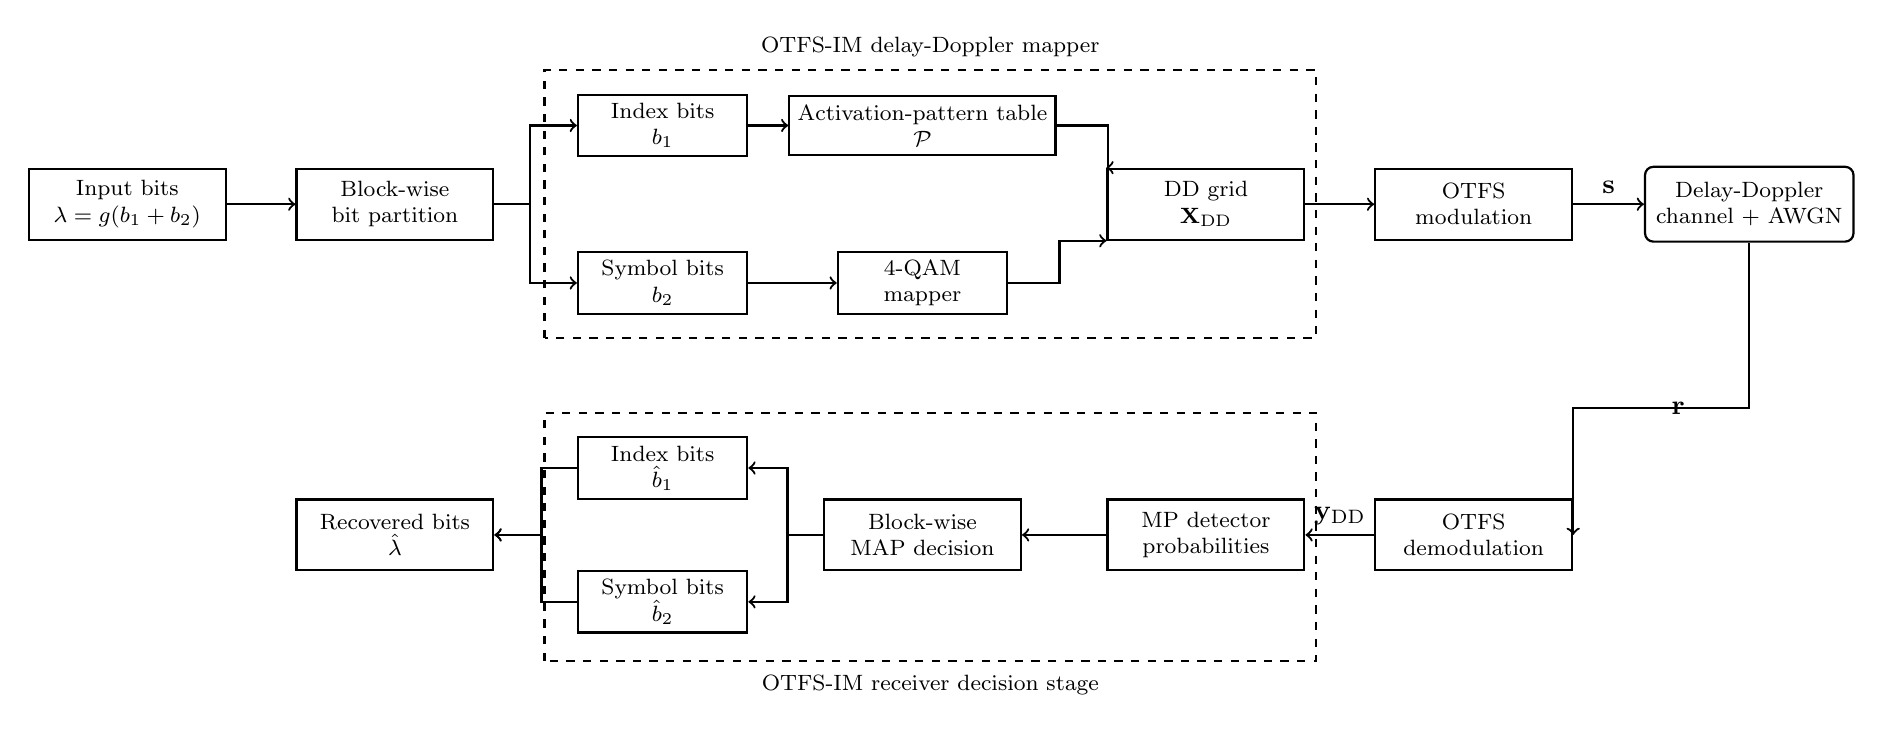
\begin{tikzpicture}[
        block/.style={
            rectangle,
            draw,
            thick,
            align=center,
            minimum width=2.5cm,
            minimum height=0.9cm,
            font=\footnotesize,
            inner sep=4pt
        },
        smallblock/.style={
            rectangle,
            draw,
            thick,
            align=center,
            minimum width=2.15cm,
            minimum height=0.75cm,
            font=\footnotesize,
            inner sep=3pt
        },
        channel/.style={
            rectangle,
            draw,
            thick,
            rounded corners=3pt,
            align=center,
            minimum width=2.6cm,
            minimum height=0.95cm,
            font=\footnotesize,
            inner sep=4pt
        },
        arrow/.style={->, thick}
    ]

        % Transmitter path
        \node[block] (inbits) at (0,0) {Input bits\\\(\lambda=g(b_1+b_2)\)};
        \node[block] (split) at (3.4,0) {Block-wise\\bit partition};
        \node[smallblock] (idx) at (6.8,1.0) {Index bits\\\(b_1\)};
        \node[smallblock] (sym) at (6.8,-1.0) {Symbol bits\\\(b_2\)};
        \node[smallblock] (map) at (10.1,1.0) {Activation-pattern table\\\(\mathcal{P}\)};
        \node[smallblock] (qam) at (10.1,-1.0) {4-QAM\\mapper};
        \node[block] (ddgrid) at (13.7,0) {DD grid\\\(\mathbf{X}_{\mathrm{DD}}\)};
        \node[block] (mod) at (17.1,0) {OTFS\\modulation};
        \node[channel] (chan) at (20.6,0) {Delay-Doppler\\channel + AWGN};

        % Receiver path
        \node[block] (demod) at (17.1,-4.2) {OTFS\\demodulation};
        \node[block] (mp) at (13.7,-4.2) {MP detector\\probabilities};
        \node[block] (mapdet) at (10.1,-4.2) {Block-wise\\MAP decision};
        \node[smallblock] (idxrx) at (6.8,-3.35) {Index bits\\\(\hat{b}_1\)};
        \node[smallblock] (symrx) at (6.8,-5.05) {Symbol bits\\\(\hat{b}_2\)};
        \node[block] (outbits) at (3.4,-4.2) {Recovered bits\\\(\hat{\lambda}\)};

        % Transmitter arrows
        \draw[arrow] (inbits.east) -- (split.west);
        \draw[arrow] (split.east) -- ++(0.45,0) |- (idx.west);
        \draw[arrow] (split.east) -- ++(0.45,0) |- (sym.west);
        \draw[arrow] (idx.east) -- (map.west);
        \draw[arrow] (sym.east) -- (qam.west);
        \draw[arrow] (map.east) -- ++(0.65,0) |- (ddgrid.north west);
        \draw[arrow] (qam.east) -- ++(0.65,0) |- (ddgrid.south west);
        \draw[arrow] (ddgrid.east) -- (mod.west);
        \draw[arrow] (mod.east) -- node[above] {\(\mathbf{s}\)} (chan.west);

        % Receiver arrows
        \draw[arrow] (chan.south) -- ++(0,-2.1) -| node[pos=0.25, right] {\(\mathbf{r}\)} (demod.east);
        \draw[arrow] (demod.west) -- node[above] {\(\mathbf{y}_{\mathrm{DD}}\)} (mp.east);
        \draw[arrow] (mp.west) -- (mapdet.east);
        \draw[arrow] (mapdet.west) -- ++(-0.45,0) |- (idxrx.east);
        \draw[arrow] (mapdet.west) -- ++(-0.45,0) |- (symrx.east);
        \draw[arrow] (idxrx.west) -- ++(-0.45,0) |- (outbits.east);
        \draw[arrow] (symrx.west) -- ++(-0.45,0) |- (outbits.east);

        \draw[dashed, thick] (5.3,-1.7) rectangle (15.1,1.7);
        \node[font=\footnotesize] at (10.2,2.0) {OTFS-IM delay-Doppler mapper};
        \draw[dashed, thick] (5.3,-5.8) rectangle (15.1,-2.65);
        \node[font=\footnotesize] at (10.2,-6.1) {OTFS-IM receiver decision stage};

    \end{tikzpicture}
    }
    \caption{Overall architecture of the implemented OTFS-IM transceiver}
    \label{fig:otfs_im_transceiver_architecture}
\end{figure}

\subsubsection{Design Scope and Relation to the Baseline OTFS System}

The OTFS-IM design in this chapter is built deliberately on top of the baseline OTFS system. The baseline system already defines the delay-Doppler grid, the modulation and demodulation operations, the channel model, and the MP detector. Chapter 4 therefore focuses only on the components that are new to OTFS-IM: block-wise mapping, activation-pattern tables, pattern selection, and block-wise receiver decisions.

This separation avoids unnecessary repetition. The ISFFT, Heisenberg transform, Wigner transform, SFFT, and delay-Doppler input-output model have already been developed in Chapter 3. In this chapter, these blocks are treated as established processing stages. The emphasis is instead placed on how the delay-Doppler input grid is constructed differently and how the receiver interprets the probability output of the detector differently.

The system considered in this thesis is an uncoded OTFS-IM system with perfect channel-state information at the receiver. Channel coding, channel estimation, synchronization errors, and standardized vehicular channel profiles are not included in the Chapter 4 design. These assumptions are consistent with the baseline model in Chapter 3 and are chosen to isolate the effect of index modulation and activation-pattern selection. Adding more practical impairments would make it harder to determine whether the observed performance difference comes from OTFS-IM itself or from another system component.

The design scope also differs from some OTFS-IM studies that focus mainly on new detector architectures such as MMSE-based or vector-wise message passing detectors. In this thesis, the receiver uses the existing MP detector as a probability engine and adds a block-wise MAP decision stage for OTFS-IM. This choice keeps the receiver structure close to the baseline OTFS system while still allowing the thesis to evaluate the reliability of index detection. The main contribution is therefore not a completely new OTFS detector, but a controlled OTFS-IM simulation framework with deterministic activation-pattern selection and detailed error-component analysis.

This design direction leads naturally to the rest of the chapter. Section 4.2 defines the IM block and spectral-efficiency calculation. Section 4.3 introduces the activation-pattern table. Section 4.4 describes the OTFS-IM transmitter. Section 4.5 presents the receiver and block-wise MAP detection process. Section 4.6 then develops the OHD and Balanced-OHD pattern-selection methods used to construct reliable activation-pattern tables.
